\chapter{Network Training}
\section{Backpropagation in Neural Networks}


\begin{figure}[H]
    \centering
    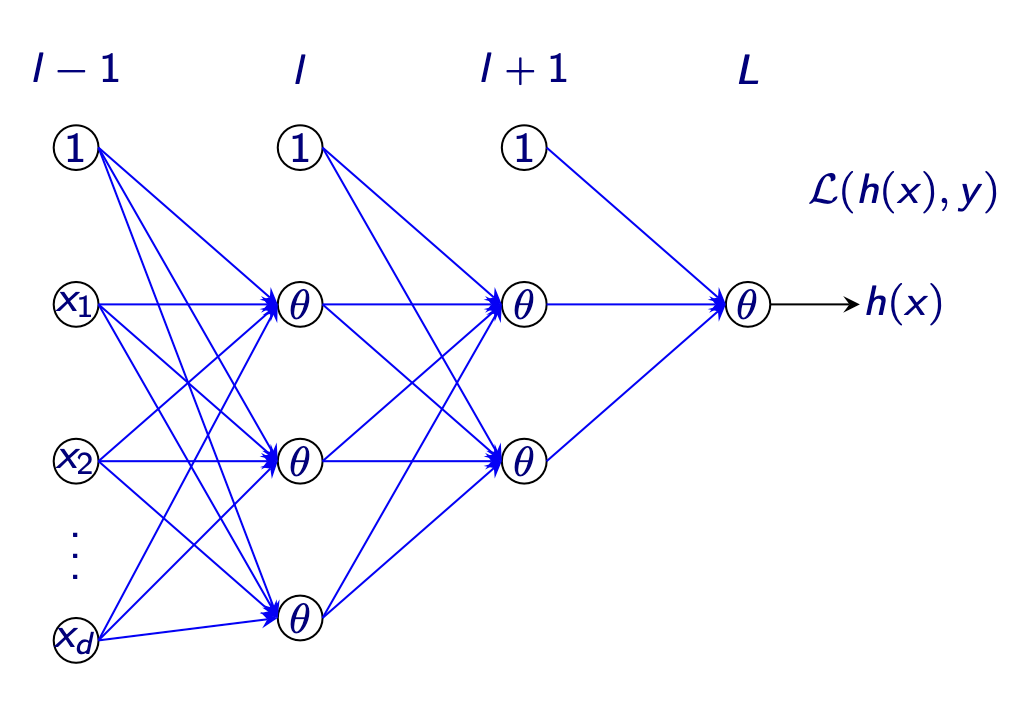
\includegraphics[width=0.55\linewidth]{img/nn.png}
\end{figure}

\begin{itemize}
    \item \textbf{Weights} are denoted as \( W^{(l)} \) for layer \( l \), with \( W_{ij}^{(l)} \) representing the weight from the \( i \)-th neuron in layer \( l-1 \) (input) to the \( j \)-th neuron in layer \( l \) (output). The layer indexing runs from 1 to \( L \) where \( L \) is the total number of layers.
    \item The \textbf{input} vector \( x \) applied to the input layer, represented as \( x^{(0)} \) with components \( x_1^{(0)}, \ldots, x_{d^{(0)}}^{(0)} \), leads to the output \( x_1^{(L)} = h(x) \in \mathbb{R} \), where \( h(x) \) is the hypothesis function.
    \item \textbf{Activations} (outputs) of layer \( l \) are denoted as \( x_j^{(l)} \), which are computed using an activation function \( \theta \) applied to the pre-activation values \( s_j^{(l)} \). This can be expressed as:
    \[ x_j^{(l)} = \theta(s_j^{(l)}) = \theta \left( \sum_{i=0}^{d^{(l-1)}} W_{ij}^{(l)} x_i^{(l-1)} \right) \]
    where \( d^{(l-1)} \) and \( d^{(l)} \) are the number of inputs and outputs for layer \( l \), respectively.
    \item The \textbf{diagonal matrix of activations} at layer \( l \), denoted as \( \Theta^{(l)} \), is the diagonal matrix containing the activation function derivatives and can be calculated as:
    \[ \Theta^{(l)} = \text{diag}(\theta'(s^{(l)})) \]
    which is a square matrix with dimensions equal to the number of outputs of layer \( l \).
    \item The \textbf{gradient} with respect to the pre-activation values \( s^{(l)} \) is given by \( \delta^{(l)} \), which is used in the backpropagation algorithm to compute the gradient of the loss function with respect to the weights \( W^{(l)} \).
\end{itemize}


\begin{definitionbox}{Gradient}
The gradient \( \delta^{(l)} \) for layer \( l \) in a neural network during backpropagation is given by:
\[ \delta^{(l)} = \left( \prod_{k=l}^{L-1} \Theta'(s^{(k)})W^{(k)T} \right)\Theta'(s^{(L)}) \nabla_{x^{(L)}} \mathcal{L} \]
where \( \Theta'(s^{(l)}) \) is the derivative of the activation function evaluated at the pre-activation level \( s^{(l)} \), \( W^{(k)} \) are the weights of layer \( k \), and \( \nabla_{x^{(L)}} \mathcal{L} \) is the gradient of the loss \( \mathcal{L} \) with respect to the activations of the last layer \( x^{(L)} \).

The update rule for the weights is then:
\[ \Delta W^{(l)} = \nabla_W \mathcal{L} = -\eta x^{(l-1)} \delta^{(l)} \]
which includes the learning rate \( \eta \), and requires forward propagation to obtain the error \( \mathcal{L} \).
\end{definitionbox}

\section{The Problem of Vanishing and Exploding Gradients}

The vanishing and exploding gradient problem is a significant challenge in training deep neural networks. It occurs during backpropagation, described as:
\[ \delta^{(l)} = \left( \prod_{k=l}^{L-1} \Theta'(s^{(k)})W^{(k)T} \right)\Theta'(s^{(L)}) \nabla_{x^{(L)}} \mathcal{L} \]
where \( \delta^{(l)} \) represents the gradient at layer \( l \), \( \Theta'(s^{(k)}) \) is the derivative of the activation function at the pre-activation values \( s^{(k)} \), and \( W^{(k)} \) is the weight matrix for layer \( k \).

\begin{itemize}
    \item Activation functions like sigmoid or tanh can saturate, which means their derivatives can become very small. Consequently, during backpropagation, these small derivatives multiply together exponentially with depth, leading to very small gradients. This is known as the \textbf{vanishing gradient} problem, which results in slow or stagnant learning.
    \item On the other hand, if the weight matrices have large eigenvalues, the gradients can grow exponentially as they backpropagate through the layers, leading to the \textbf{exploding gradient} problem, where weight updates are so large they can cause the learning process to diverge.
    \item Deep networks are particularly susceptible to these issues due to their depth and complexity.
\end{itemize}

\subsection*{Intuitive Explanation}
Consider the backpropagation of errors in a deep network as a process of transmitting signals. If the transmission channel (represented by the activation functions and weight matrices) weakens the signal too much (vanishing gradients), the information about the error doesn't reach the earlier layers effectively. This is similar to whispering a message across a long chain of people– by the time it reaches the end, the message might be lost.\\

Conversely, if the channel amplifies the signal too much (exploding gradients), the information about the error overshoots its target, leading to large, erratic updates. This is akin to using a megaphone for the same message in a small room; the message doesn't just reach the intended person but bounces around the walls, creating chaos.

\subsection*{Mitigation Strategies}
To address these problems, several strategies are employed:
\begin{itemize}
    \item \textbf{Network Design:} Architectural choices, such as using shorter connections (skip connections) that allow gradients to bypass certain layers directly.
    \item \textbf{Initialisation:} Careful initialisation of the weights to ensure that the eigenvalues of the weight matrices are neither too small nor too large.
    \item \textbf{Regularisation:} Techniques such as gradient clipping are used to prevent gradients from becoming too large.
\end{itemize}


\begin{definitionbox}{Epoch}
An \textbf{Epoch} represents a single pass through the entire dataset, where each example in the dataset has been used once for both forward and backward propagation. Typically, a single epoch is not sufficient for convergence; the model may require multiple epochs to adequately learn from the data. As the number of epochs increases, the model's performance on training data usually improves, from underfitting to optimal fitting, and can eventually lead to overfitting. The appropriate number of epochs can vary widely between different datasets.
\end{definitionbox}

\begin{definitionbox}{Batch}
A \textbf{Batch} refers to the subset of the dataset that is processed together in one iteration of training. The entire dataset is divided into a number of these batches. The \textbf{Batch Size} is the number of training examples in a single batch. It is important to distinguish between batch size and the number of batches, which are related but not the same—the number of batches is determined by dividing the total number of examples by the batch size.
\end{definitionbox}

\begin{definitionbox}{Iteration}
An \textbf{Iteration} is one update of the model's parameters, which is done after processing a batch. The number of iterations needed to complete one epoch is equal to the number of batches in the dataset. Therefore, the number of iterations for one epoch is the total number of examples divided by the batch size.
\end{definitionbox}

\section{Reducing Overfitting}

There are several measures we can take to reduce overfitting in models. This is usually because the network is too large, it has been trained too long on the data, or a lack of data points.

\subsection*{Remedies}
\begin{itemize}
    \item Reduce network complexity, less layers
    \item Regularisation 
        \begin{itemize}
            \item Momentum and weight decay
            \item Dropout
            \item Weight initialisation
            \item Batch normalisation
        \end{itemize}
    \item Data augmentation
    \item Patience/early stopping
    \item Weight sharing
    \item Ensemble predictions (pattern recognition)
    \item Multitask learning
    \item Adversarial training (hard negatives)
\end{itemize}

\section{Optimisers}
\begin{commentbox}{Notation: Hadamard Product}
    We use \(\odot\) to refer to the Hadamard product, which consists of element-wise multiplication. The Hadamard product is associative and distributive. Unlike the matrix product, it is also commutative.

    \[
\begin{bmatrix}3&5&7\\4&9&8\end{bmatrix}\odot\begin{bmatrix}1&6&3\\0&2&9\end{bmatrix}=\begin{bmatrix}3\times1&5\times6&7\times3\\4\times0&9\times2&8\times9\end{bmatrix}
    \]
    
\end{commentbox}
\subsection{Stochastic Gradient Descent (Mini batch)}

\begin{definitionbox}{Mini-batch Stochastic Gradient Descent (SGD)}
Mini-batch Stochastic Gradient Descent (SGD) is an optimisation technique used to train neural networks by updating the model's weights based on the gradient of the loss function with respect to the weights. Key components of mini-batch SGD include:

\begin{itemize}
    \item \textbf{Loss Function}: The average loss over a mini-batch is given by
    \[ \mathcal{L} = \frac{1}{n} \sum_{i} \ell(h(x_i), y_i) \]
    where \( \ell \) is the loss for a single data point, \( h(x_i) \) is the hypothesis function evaluated at input \( x_i \), and \( y_i \) is the true label.

    \item \textbf{Gradient of the Loss}: The gradient with respect to the weights \( W \) is
    \[ \nabla_W \mathcal{L} = \frac{1}{n} \sum_{i} \nabla_W \ell(h(x_i), y_i) \]

    \item \textbf{Weight Update}: The weights are updated by moving in the negative direction of the gradient, scaled by the learning rate \( \eta \):
    \[ W_{t+1} = W_t - \eta \nabla_W \mathcal{L}_t \]

    \item \textbf{Learning Rate \( \eta \)}: This hyperparameter controls the step size during the weight update. It plays a crucial role in convergence and must be carefully tuned. A learning rate that is too high can cause the training to diverge, while a rate that is too low results in slow convergence.

    \begin{figure}[H]
    \centering
    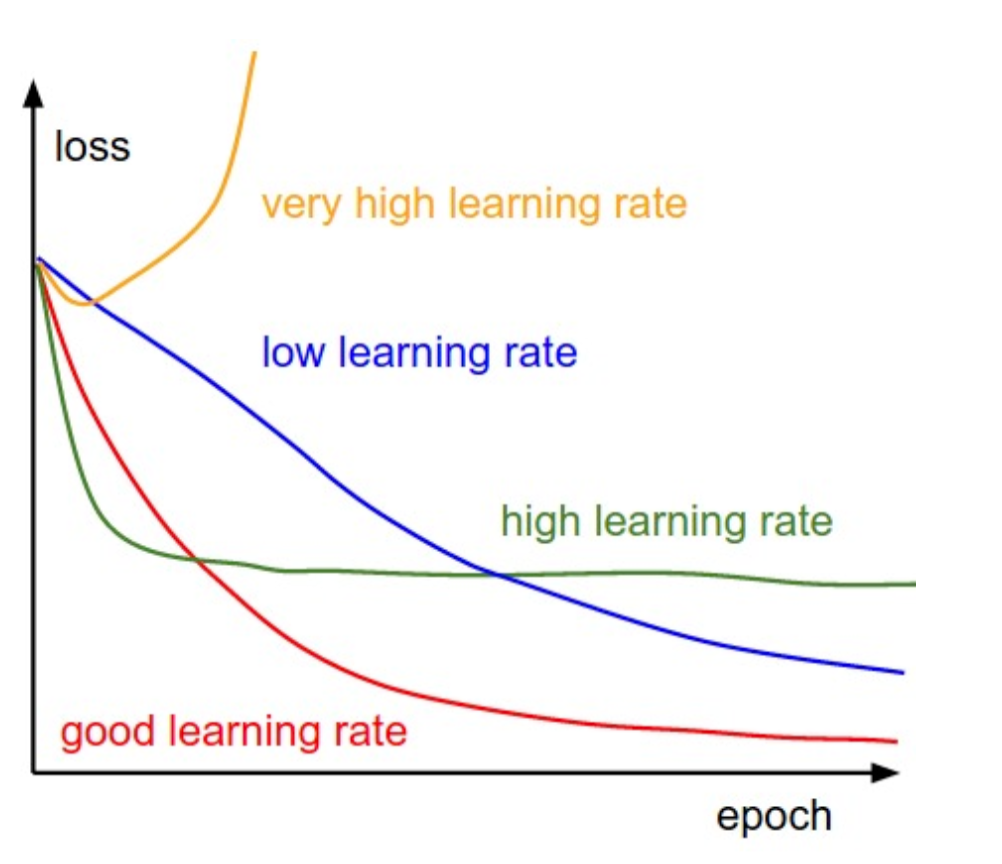
\includegraphics[width=0.5\linewidth]{img/sgd_learnrate.png}
    \caption{Graph showing a loss over epochs for different learning rates}
    \end{figure}
\end{itemize}

Convergence can be slow with mini-batch SGD, and selecting an appropriate learning rate often requires experimentation. Learning rate schedules or adaptive learning rate methods are used to adjust \( \eta \) during training to improve convergence.
\end{definitionbox}



\begin{definitionbox}{SGD with momentum (mini-batch)}


SGD with momentum is a variation of the standard SGD that accelerates convergence by incorporating a fraction of the previous weight update. Loss is defined by:

\[ \mathcal{L} = \frac{1}{n} \sum_{i} \ell(h(x_i), y_i) \]
where \( h(x_i) \) is the hypothesis function for input \( x_i \) and \( y_i \) is the true value. The gradient of the loss with respect to the weights is:
\[ \nabla_w \mathcal{L} = \frac{1}{n} \sum_{i} \nabla_w \ell(h(x_i), y_i) \]
Weights are updated by subtracting a fraction of the gradient, controlled by the learning rate \( \eta \):
\[ W_{t+1} = W_t - \eta \nabla_w \mathcal{L}(W_t) \]

It introduces the momentum term \( \beta \) which determines the contribution of past gradients to the current direction:
\[ Z_{t+1} = \beta Z_t + \nabla_w \mathcal{L}(W_t) \]

Momentum accumulates with past updates.\\


The weight update rule is then modified to:
\[ W_{t+1} = W_t - \eta Z_{t+1} \]
where \( \beta \) typically has a value around 0.9. When \( \beta = 0 \), this reduces to the standard SGD. The momentum term helps in smoothing out the updates and can lead to faster convergence.

\begin{figure}[H]
    \centering
    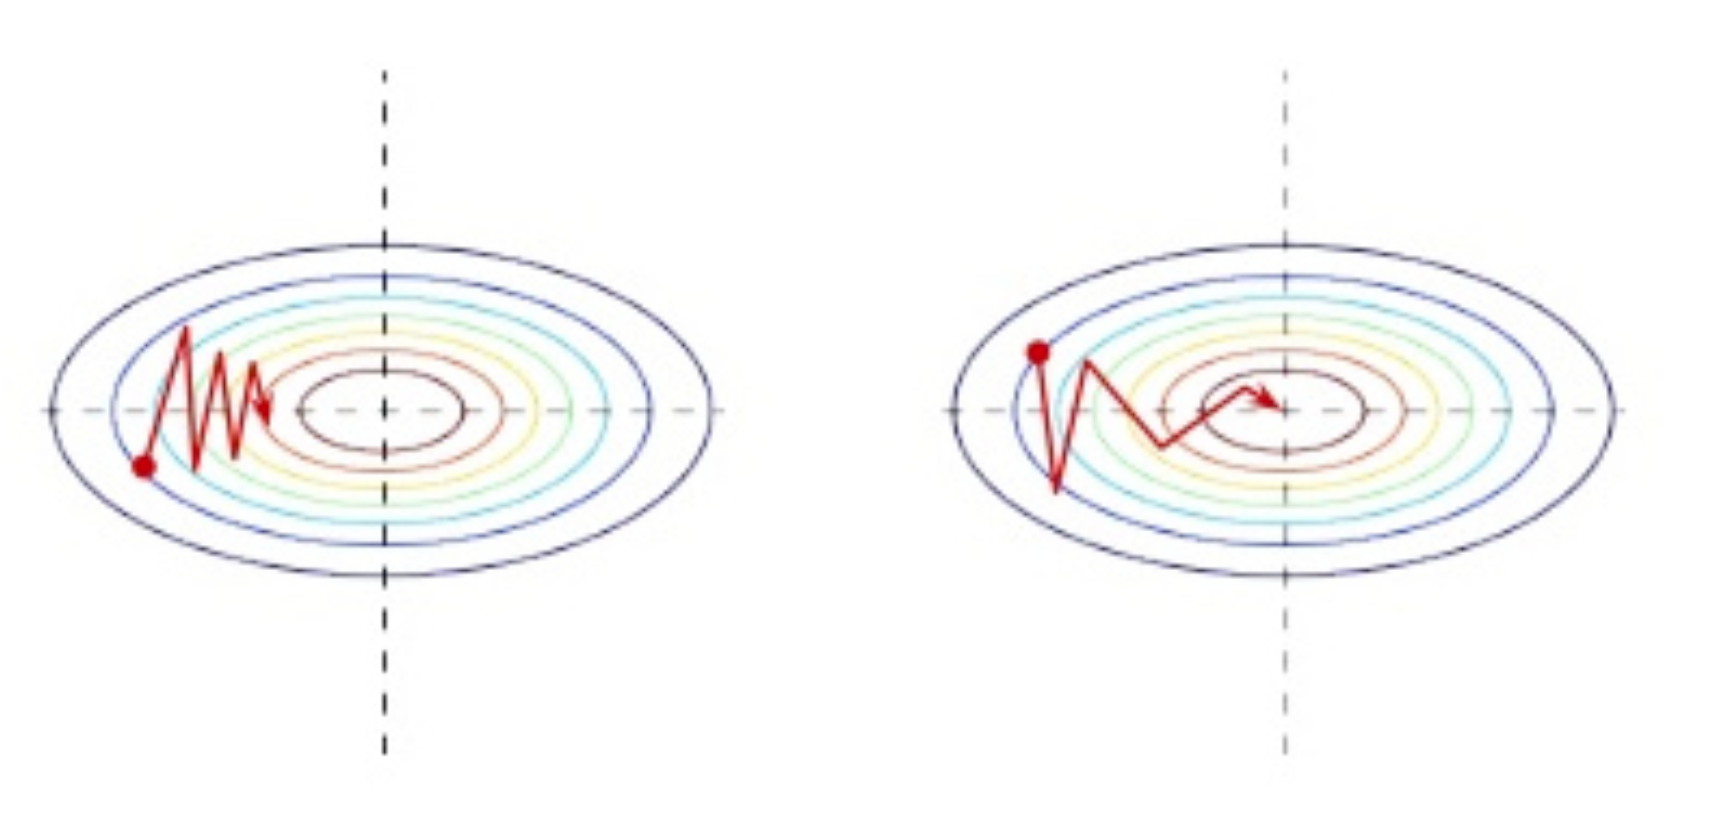
\includegraphics[width=0.5\linewidth]{img/sgd_mom.png}
    \caption{For momentum-based SGD, for any component where the gradient is heading in the intended direction, momentum is accumulated in that direction. In this example, note a horizontal acceleration towards the centre.}
    
\end{figure}
\end{definitionbox}

\begin{definitionbox}{SGD with Nesterov momentum}
Stochastic Gradient Descent (SGD) with Nesterov momentum is an optimisation technique that aims to accelerate SGD by taking into account the direction of the previous gradient step. It is described as follows:
\begin{itemize}
    \item The loss \( \mathcal{L} \) is computed as the average of the loss function \( \ell \) over all examples \( x_i \) in the mini-batch:
    \[ \mathcal{L} = \frac{1}{n} \sum_{i} \ell(h(x_i), y_i) \]
    \item The gradient of the loss with respect to the weights is:
    \[ \nabla_w \mathcal{L}(W) = \frac{1}{n} \sum_{i} \nabla_w \ell(h(x_i), y_i) \]
    \item The Nesterov momentum update is defined as:
    \[ Z_{t+1} = \beta Z_t + \nabla_w \mathcal{L}(W_t - \eta\beta Z_t) \]
    Note the lookahead step occurring in the loss function. Compare this to basic momentum given by:
    \[ Z_{t+1} = \beta Z_{t} + \nabla_w \mathcal{L}(W_t) \]
    Nesterov momentum involves calculating the decaying moving average of the gradients of projected positions in the search space rather than the actual positions themselves.


    \item The weight update formula is then:
    \[ W_{t+1} = W_t - \eta Z_{t+1} \]
\end{itemize}
Nesterov momentum improves upon standard momentum by refining the direction of the step not only with the current gradient but also by looking ahead at where the next step would take the optimisation process. This anticipatory update prevents us from going too fast and results in more responsive gradient steps.

Nesterov momentum involves:
\begin{enumerate}
    \item Making a step in the direction of the accumulated gradient.
    \item Measuring the gradient in this new point and correct the direction.
\end{enumerate}
This approach can significantly accelerate the convergence of SGD, especially in the context of high curvature, noisy gradients, or small mini-batches.
\begin{figure}[H]
    \centering
    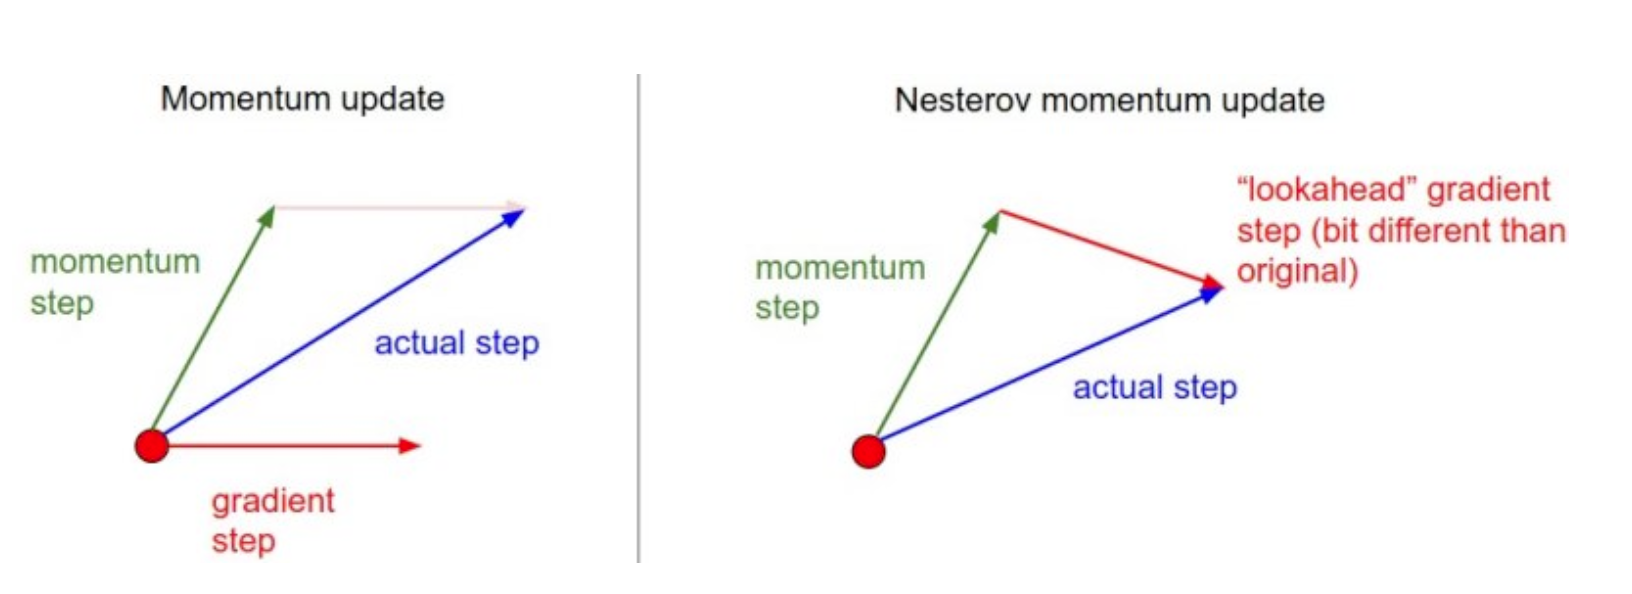
\includegraphics[width=0.7\linewidth]{img/nesterov.png}
    \caption{Lookahead gradient visualisation}
    
\end{figure}
\end{definitionbox}

\begin{definitionbox}{Adagrad}
Adagrad is an optimisation algorithm designed to adapt the learning rate to the parameters, performing smaller updates for parameters associated with frequently occurring features, and larger updates for parameters associated with infrequent features. It is particularly well-suited for dealing with sparse data. The Adagrad update rule is defined as follows:
\begin{itemize}
    \item The weight update rule is:
    \[ W_{t+1} = W_t - \frac{\eta}{\sqrt{G_t + \epsilon}} \odot \nabla_w \mathcal{L}(W_t) \]
    where \( G_t \in \mathbb{R}^{p \times p} \) is a diagonal matrix where each diagonal element \( i, i \) is the sum of the squares of the gradients with respect to \( w_i \) up to iteration \( t \), \( \eta \) is the learning rate, and \( \epsilon \) is a small smoothing term to prevent division by zero.
    \item Adagrad adapts the learning rate for each parameter, reducing the learning rate monotonically for each parameter.
    \item It has been used effectively in training GloVe word embeddings, among other applications.
    \item However, the monotonic decrease can sometimes lead to premature and excessive reduction in the effective learning rate, causing the algorithm to stop learning.
\end{itemize}

Intuitively, we are trying to step the weights vector through a (generally high) dimensional space trying to minimise the loss function. This is done by moving in the opposite direction to gradient. However, not all dimensions are equal. Some consistently receive larger gradients, some receive smaller gradients. If we use a uniform learning rate, we might step too far in directions with large gradients (potentially overshooting the minimum), and too little with small gradients (taking too long to converge). The diagonal matrix \(G\) is used to keep track of historical gradients, serving as an automatic tuning dial for learning rates.
\end{definitionbox}

\begin{definitionbox}{RMSProp}
RMSProp (Root Mean Square Propagation) is an adaptive learning rate method that adjusts the learning rate for each weight individually. It modifies the general gradient descent weight update rule as follows:
\begin{itemize}
    \item The weight update rule is:
    \[ W_{t+1} = W_t - \frac{\eta}{\sqrt{E[\nabla \mathcal{L}^2]_t + \epsilon}} \odot \nabla_w \mathcal{L}(W_t) \]
    \item The expected squared gradient \( E[\nabla \mathcal{L}^2]_t \) is the exponentially decaying average of squared gradients:
    \[ E[\nabla \mathcal{L}^2]_t = \gamma E[\nabla \mathcal{L}^2]_{t-1} + (1 - \gamma)(\nabla \mathcal{L}_t)^2 \]
\end{itemize}
Intuitively, RMSProp uses the magnitude of recent gradients to normalised the gradient; this is akin to adjusting the step size depending on the 'steepness' of the learning landscape. It prevents oscillations in directions with large gradients and allows for faster progress in directions with small gradients.
\end{definitionbox}

\begin{definitionbox}{Adadelta}
Adadelta is an extension of Adagrad that seeks to reduce its aggressive, monotonically decreasing learning rate. Instead of accumulating all past squared gradients, Adadelta limits the window of accumulated past gradients to some fixed size. The update rule is:
\begin{itemize}
    \item The weight update rule is:
    \[ W_{t+1} = W_t - \frac{\sqrt{E[\Delta W^2]_{t-1} + \epsilon}}{\sqrt{E[\nabla \mathcal{L}^2]_t + \epsilon}} \odot \nabla_w \mathcal{L}(W_t) \]
    \item The update accumulation \( E[\Delta W^2]_t \) is computed as:
    \[ E[\Delta W^2]_t = \gamma E[\Delta W^2]_{t-1} + (1 - \gamma)(W_t - W_{t-1})^2 \]
\end{itemize}
Intuitively, Adadelta adapts the learning rate based on a moving window of gradient updates, rather than accumulating all past squared gradients. This allows the learning rate to remain more robust and not decay to infinitesimally small values, which addresses the vanishing learning rate problem of Adagrad.
\end{definitionbox}

\begin{definitionbox}{Adam (Adaptive Moment Estimation)}
Adam is an optimisation algorithm that computes adaptive learning rates for each parameter by estimating the first and second moments of the gradients. Its update rule combines the advantages of two other extensions of stochastic gradient descent, AdaGrad and RMSProp. Specifically, the Adam update rule is given by:
\begin{itemize}
    \item The weight update rule is:
    \[ W_{t+1} = W_t - \frac{\eta}{\sqrt{v_t + \epsilon}} \odot m_t \]
    \item The first moment \( m_t \) and second moment \( v_t \) estimates are:
    \[ m_t = \frac{\beta_1 m_{t-1} + (1 - \beta_1) \nabla_w \mathcal{L}_t}{1 - \beta_1^t} = \frac{\mathbb{E}\left[ \nabla_w \mathcal{L}_t\right]}{1 - \beta_1^t} \]
    \[ v_t = \frac{\beta_2 v_{t-1} + (1 - \beta_2) (\nabla_w \mathcal{L}_t)^2}{1 - \beta_2^t} = \frac{\mathbb{E}\left[ \nabla_w \mathcal{L}_t\right]}{1 - \beta_1^t} \]
\end{itemize}
Intuitively, Adam performs smaller updates for parameters associated with frequently occurring features and larger updates for parameters associated with infrequent features. It uses the squared gradients to scale the learning rate and takes advantage of momentum by using the moving average of the gradient. It corrects for the initial bias towards zero in the first and second moment estimates, providing a more accurate update step.

Commonly used values for the decay parameters are \( \beta_1 \approx 0.9 \), \( \beta_2 \approx 0.999 \), and \( \epsilon \approx 10^{-8} \), which control the exponential decay rates for these moment estimates.
\end{definitionbox}

\subsection{Comparison of Optimisers}
\begin{figure}[H]
    \centering
    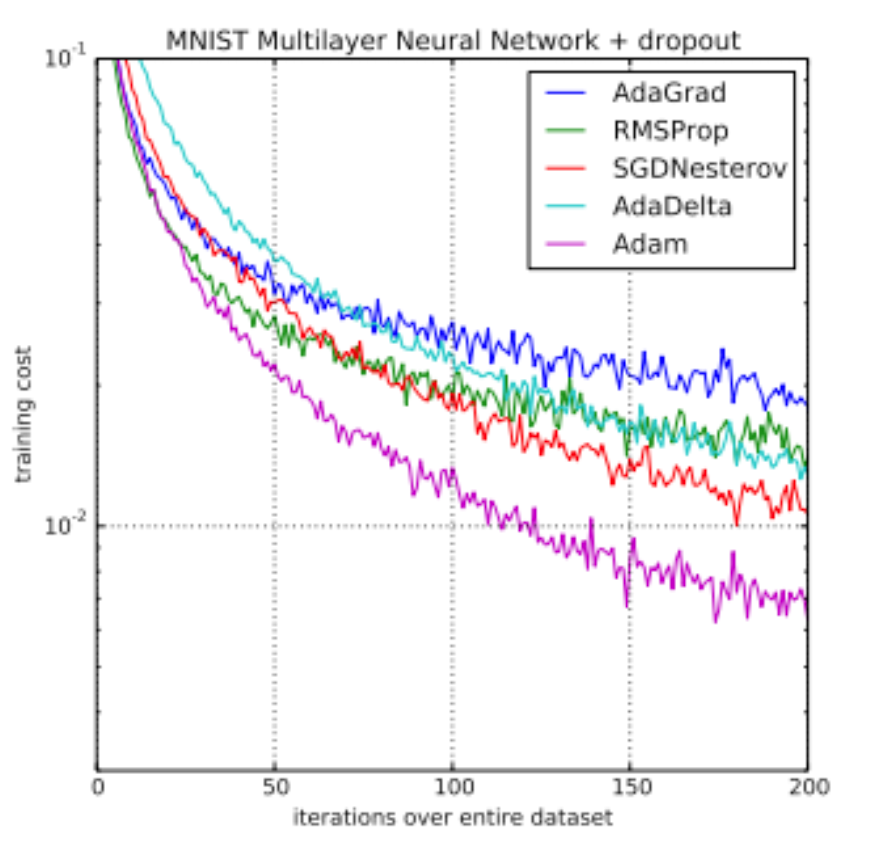
\includegraphics[width=0.5\linewidth]{img/optimisers.png}
    \caption{Comparison of training cost over iterations for different optimisers]}
    
\end{figure}

\begin{itemize}
    \item Adagrad introducing an adaptive learning rate, best suited for sparse data.
    \item RMSProp resolves vanishing learning rates by using decaying averages
    \item Adadelta is similar to RMSProp but does not require a learning rate
    \item Adam is RMSProp + Momentum, also adds bias correction
    \item SGD is often used, tends to find a good minimiser and generalises well
\end{itemize}

\section{Regularisation}
\subsection{Dropout}
\subsection{Distribution Problem}
\subsection{Batch Normalisation}
\section{Network Design}
\subsection{Baseline}
\subsection{Finetuning}
\subsection{Data Collection}
\subsection{Validation}
\subsection{Data Augmentation}
\subsection{Adversarial Training}
\subsection{Setting Parameters}
\subsection{Monitoring and Debugging}




